\section{Analysis and results}
\label{sec:results}

\begin{table*}[t]
    \centering
    \begin{threeparttable}
    \begin{tabular}{||l|c|c|r||}
        \toprule
            Node type & Complexity & Memory cost & Communication cost \\
        \midrule \midrule
		    Prover & $O(n^2log(n))$ & $160+10*s$ & \vtop{\hbox{\strut (send) $32*g + 94$}\hbox{\strut (recv) $64 + 96 * h$}} \\
		\midrule
		    Aggregator & $O(n log(n))$ & $276+10*s+96*z$ & \vtop{\hbox{\strut (send) $(32*c+94)*nb + 64 + 96*z$}\hbox{\strut (recv) $(32*c+94) + 96* nb + 96*z$}} \\
		\midrule
		    Verifier & $O(n^2log(n))$ & - & - \\
		\midrule
	\end{tabular}
	\begin{tablenotes}
	    \item[1] n = number of bits in input
	    \item[2] z = number of bad neighbours
		\item[3] c = number of counters
    \end{tablenotes}
    \caption{\todo{table caption}}
    \label{tab:1}
    \end{threeparttable}
\end{table*}



\subsection{Computational cost}
\todo{here describe the computational cost and make a parallel with original
SANA (is it the same?)}
We now proceed to evaluate the computational, memory and communication costs of SANA for Provers and Aggregators since we can't make assumption on their costs and the algorithm needs to be feasible even for low-end devices.
Starting from the computational cost we can see that the most complex functions of the protocol are the sign and verify functions as they both have to perform operations on the elliptic curve that require several multiplication to be executed.
Table~\ref{tab:1} report our estimations for the computational costs of the functions related to the nodes using them, for evaluating this costs we refer to the variable n which is the number of bits of the input given to the function, in our case n = 256 bits.
So we can safely say that the highest cost falls on the provers while the aggregators, which only have to perform one multiplication between objects.
Memory costs however change the perspective of how the load is distributed over the nodes.
As we can see the memory cost for the prover is contained as long as we choose a fair amount of counters. For the aggregator instead we can see that it's sensitive to the number of bad neighbours as the node has to memorize the public key and the message of each compromised node.
We evaluated more in depth the problem of the aggregator by running tests to determine the effective memory cost based on the number of compromised deviced nearby each node

At last we evaluated the theoretical communication costs for the protocol, based on the bytes each actor has to send or receive.
As for the memory cost the aggregator has to send and receive more bytes depending on how many compromised devices the aggregator has as its neighbours

With this theoretical results in mind we looked more in depth at the memory cost by looking at how much the number of bad neighbour would impact the aggregators, the results are shown in section \ref{sec:results}.

After dealing with the theoretical costs we shifted to the practical test in order to estimate the true work load for the nodes.
We ran several simulation to investigate the time required to perform each action of the protocol (signature, aggregation, verify...) and have a proper estimation of the total time of execution of the algorithm.
For this calculation we used this formula:
\[(\sum_{i=0}^{n} p_i) * t_{agg} + d * (t_{ver} + t_{hash}) + t_{sign} \]
Where n is the number of the provers and d is the depth of the tree generated from the algorithm.
This provides a lower bound for the execution time of the whole protocol as it relies on the fact that all node can sign simultaneously and at each level of the tree all the challenge verifications from the aggregators require the same time.
Unfortunately this formula is not easy to use in real context as the devices move into a psace and the number of neighbour may change depending on the proximity of the other devices, so it's hard to assume what the depth of the tree can be and how much parallelization can happen while descending the tree.


\subsection{Aggregation cost}
For what concerns the duration of the process of aggregation we extracted the aggregation time of 1 aggregator with an increasing number of provers connected to him to see if our theoretical guesses are correct \ref{fig:aggregation_0}.
Firstly we can see in figure 2 the aggregation time of up to 1000 provers with 0\% of them being bad provers, this means that all of them signed the default message, theoretically we supposed that the cost in time 
for the process of aggregation wuold increase linearly with the number of provers connected to the same aggregator. We can clearly see that our supposition were correct.
Now the question was if aggregation time depends on the number of bad provers within all the provers connected to the aggregator \ref{fig:aggregation_100}.
As we supposed the percentage of bad provers do not influence the time of aggregation, in fact with 100\% bad provers (figure 3) the graph is very close to the 0\% one.\\ 
We extracted data for 0\% 25\% 50\% 75\% and 100\% of bad provers, the results in figure 4 \ref{fig:aggregation_comparison}.

\subsection{Verification cost}
The other parameter we wanted to investigate was the verification time of the aggregator with respect to the number of provers and the percentage of them not signing the default message.
Theoretically we believed that the number of bad provers would make the verification time increase linearly, and on the other hand the time of verification should be independent on the number of legitimate provers
\ref{fig:verification_0}.
In Figure 5 we can see that the time of verification is in fact independent from the number of provers if they are all legitimate \ref{fig:verification_100}.
Intsead, with 100\% of bad provers in Figure 6, the time of verification increase linearly with the number of provers, reaching up to 6000 seconds for the verification of 1000 bad provers \ref{fig:verification_compariso}.
The comparison of the verification time of 0\% 25\% 50\% 75\% 100\% bad provers is represented in Figure 7.\\

\subsection{Memory cost}
\begin{figure}
	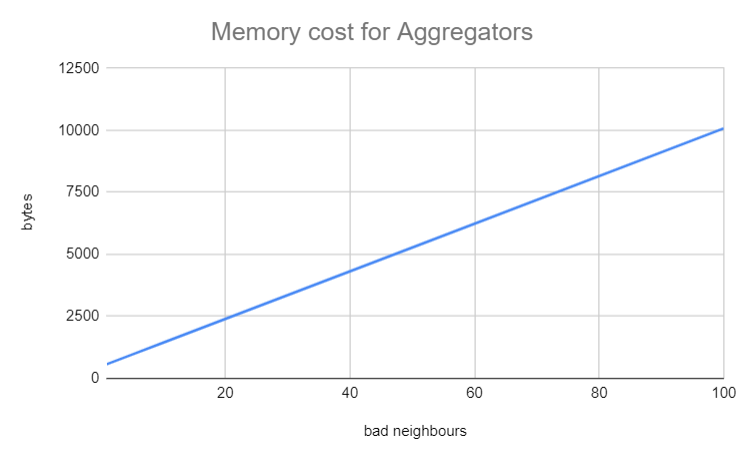
\includegraphics[width=\linewidth]{Images/memorycost.png} % Figure image
	\caption{Memory cost for the aggregator } % Figure caption
\end{figure}
In Figure 8 is represented the memory cost for the aggregator, theoretically we expected this to increase linearly with the number of bad neighbours due to the nature of the protocol identifying the compromised devices. In fact we proved this claim to be true and we can add to that the aggregator must suffer a memory cost that for the majority of low end devices is prohibiting having close to 1024Kb of memory.

\begin{figure*}
\centering
\begin{subfigure}[t]{.49\textwidth}
  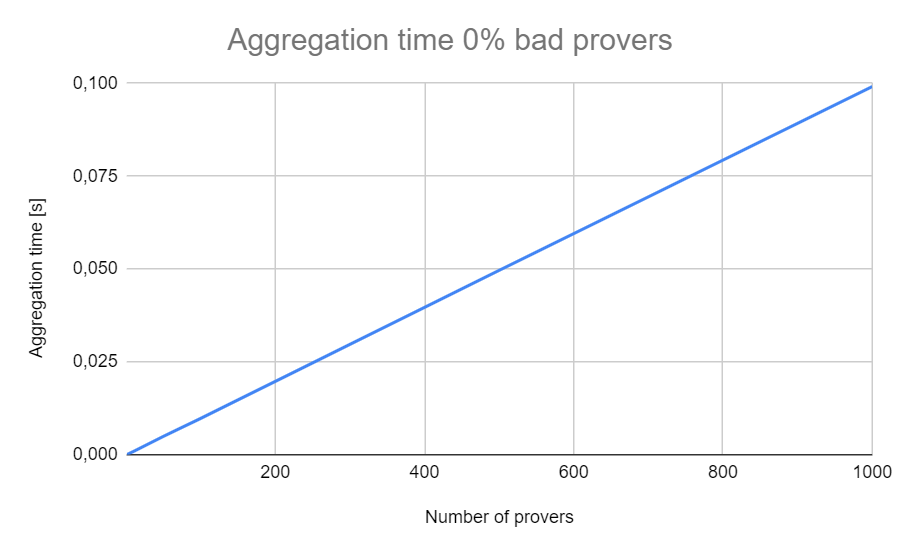
\includegraphics[width=.90\linewidth]{Images/aggregation_0.png}  
  \caption{}
  \label{fig:aggregation_0}
\end{subfigure}
\hfill
\begin{subfigure}[t]{.49\textwidth}
  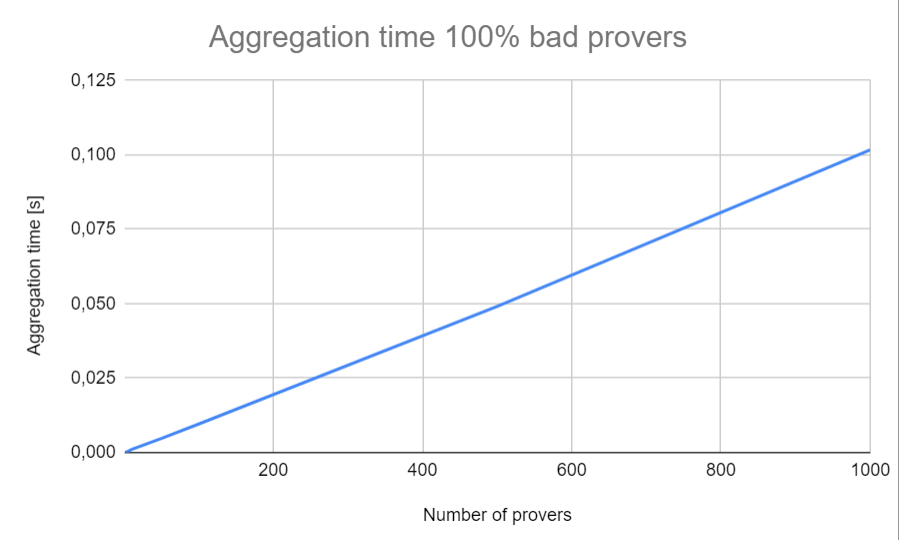
\includegraphics[width=.90\linewidth]{Images/aggregation_100.png}  
  \caption{}
  \label{fig:aggregation_100}
\end{subfigure}
\hfill
\begin{subfigure}[t]{.49\textwidth}
  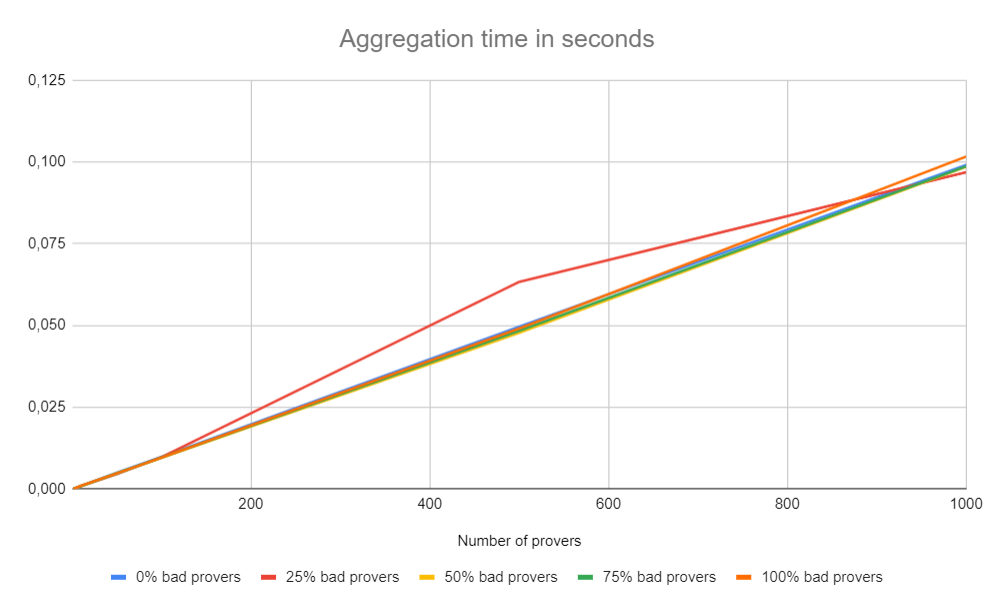
\includegraphics[width=.90\linewidth]{Images/aggregation_comparison.png}  
  \caption{}
  \label{fig:aggregation_comparison}
\end{subfigure}
\hfill
\begin{subfigure}[t]{.49\textwidth}
  \centering
  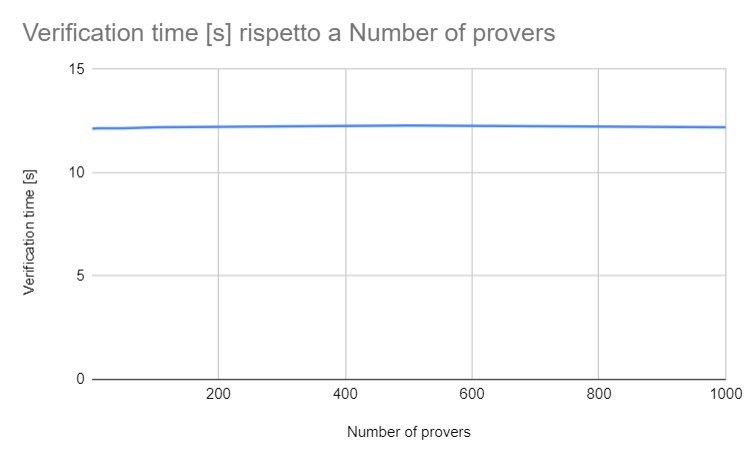
\includegraphics[width=.90\linewidth]{Images/Verification_0.png}
  \caption{}
  \label{fig:verification_0}
\end{subfigure}
\begin{subfigure}[t]{.49\textwidth}
  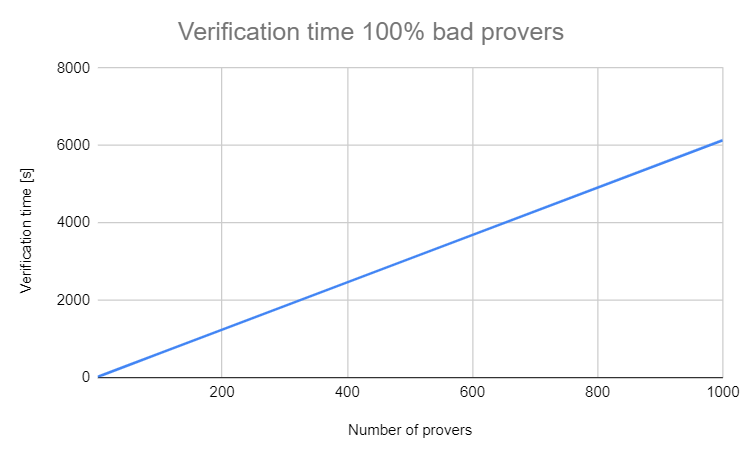
\includegraphics[width=.90\linewidth]{Images/verification_100.png}
  \caption{}
  \label{fig:verification_100}
\end{subfigure}
\hfill
\begin{subfigure}[t]{.49\textwidth}
  \centering
  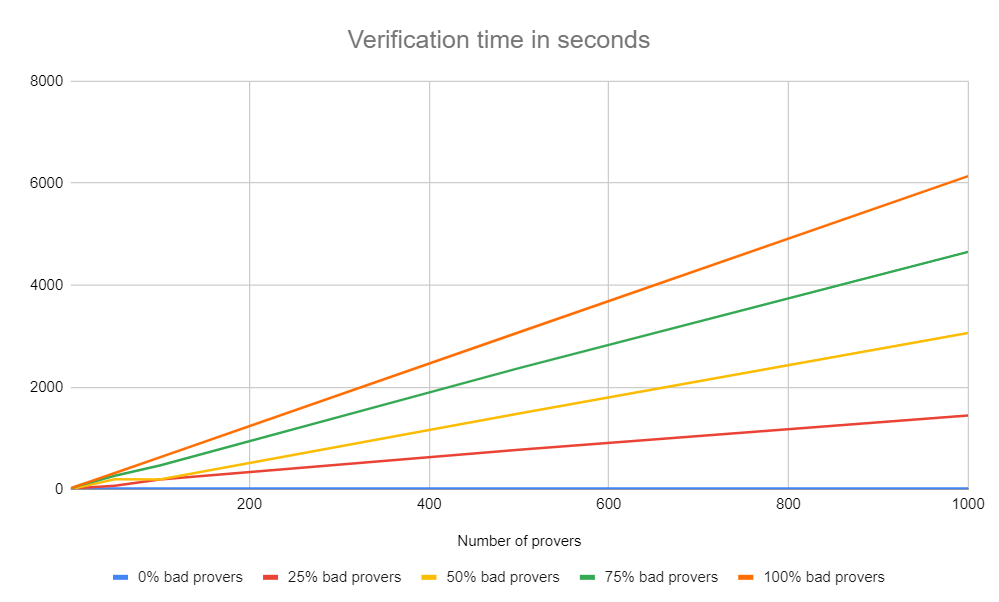
\includegraphics[width=.90\linewidth]{Images/verification_comparison.png}  
  \caption{}
  \label{fig:verification_comparison}
\end{subfigure}
\caption{\todo{general caption}}
\label{fig:prop_time}
\end{figure*}